\chapter{Multi-User Encryption}
\label{chapter:multi-user}

In the following sections the architecture and implementation of the proposed solution will be discussed, as well as some of the difficulties encountered and the corresponding solutions.

\section{Overview}
\label{sec:over-multi-user}

The purpose of this project is to enable separate encryption of various users' data under a multi-user Android environment. This means introducing the following functionalities:
\begin{itemize}
\item Choose whether a user is encrypted at creation
\item Unlock and mount encrypted data on user password entry
\item Unmount and lock encrypted data on switch user
\item Unmount and lock encrypted data on device sleep
\end{itemize}

This involves creating a framework to manage the encrypted locations (or \textit{storages}) as well as patching various Android subsystems in order to accommodate the aforementioned functionalities.

\section{Architecture}
\label{sec:arch-multi-user}

\begin{figure}[h]

\centering
\begin{tikzpicture}
[node distance = 1cm, auto,font=\footnotesize,
% STYLES
every node/.style={node distance=2cm},
comment/.style={rectangle, inner sep= 5pt, text width=3cm, node distance=1cm, align=right},
dummy/.style={rectangle, inner sep= 5pt, text width=0cm, node distance=3cm},
force/.style={rectangle, draw, fill=black!10, inner sep=5pt, text width=3cm, text badly centered, minimum height=1cm, font=\bfseries\footnotesize\sffamily}] 

% Draw forces
\node [force] (efstools) {EFS Tools};
\node [force, above of=efstools] (efsserver) {EFS Server};
\node [force, left=1cm of efstools] (openssl) {OpenSSL};
\node [force, right=1cm of efstools] (keystore) {Keystore};
\node [force, below of=efstools] (ecryptfs) {eCryptfs Module};
\node [force, below of=openssl] (secchip) {Security Chip Driver};
\node [force, above of=efsserver] (efsservice) {EFS Service};
\node [force, above of=efsservice] (keyguard) {Keyguard};
\node [force, left=1cm of efsservice] (usermanager) {UserManager Service};
\node [force, right=1cm of efsservice] (powermanager) {PowerManager Service};
\node [force, left=1cm of keyguard] (userswitcher) {User Switcher};
\node [comment, right=1cm of efsserver] (middleware) {Middleware};
\node [comment, right=1cm of ecryptfs] (kernel) {Kernel};
\node [comment, right=1cm of keyguard] (framework) {Framework};
\node [dummy, left of=openssl] (d00) {};
\node [dummy, right of=keystore] (d01) {};
\node [dummy, below=0.5cm of d00] (l00) {};
\node [dummy, below=0.5cm of d01] (l01) {};
\node [dummy, left of=usermanager] (d10) {};
\node [dummy, right of=powermanager] (d11) {};
\node [dummy, below=0.5cm of d10] (l10) {};
\node [dummy, below=0.5cm of d11] (l11) {};

\draw [dashed, thick]
	(l00) -- (l01)
	(l10) -- (l11);

% Draw the links between forces
\path[<->,very thick]
(efstools) edge (efsserver)
(efstools) edge (openssl)
(efstools) edge (keystore)
(efstools) edge (ecryptfs)
(openssl) edge (secchip)
(efsserver) edge (efsservice)
(efsservice) edge (powermanager)
(efsservice) edge (usermanager)
(efsservice) edge (userswitcher)
(efsservice) edge (keyguard);

\end{tikzpicture} 
\caption{Multi-User Encryption Architecture}
\label{fig:arch-multi-user}
\end{figure}

The architecture can be broken down into three main pieces, each containing multiple subsystems.

The first of these is the kernel layer. Here resides the eCryptfs module which has been presented in the previous chapter. Also in this layer is the security chip driver that comes into action on devices with security hardware capabilities (e.g. cryptographic acceleration).

The second component is the one where the core of the system is implemented. Called the middleware layer, it hosts the EFS Tools C library, which communicates with the OpenSSL library and the Keystore, as well as the EFS Server. EFS Tools is the C library which makes use of the kernel module to implement the management of storages. The EFS Server is a native Android service which listens on a socket for requests from the upper layer and calls the relevant EFS Tools functions.

Finally, the thrid component is situated in the Android framework. The most relevant part of it is the EFS Service, which is an Android Java Service that connects various Android subsystems to the native service and underlying C library.

Furthermore, in the framework, several Android control systems and user interfaces have been modified in order to integrate the desired functionality.

\section{C library}
\label{sec:c-multi-user}

The C library is the core component of the design. It is responsible for exposing the operations supported by the eCryptfs kernel module to the upper layers of the system.

The key notion it works with is that of \textit{secure storage} or \textit{secure container}. In this case, a secure storage is a directory in the device's file hierarchy where encrypted data is stored. It can only be mounted and accessed as a regular location with the proper credentials.

There are three main responsibilities handled by the library:
\begin{enumerate}
\item Key management
\item Container management
\item Integrity
\end{enumerate}

As discussed before, the eCryptfs kernel module encrypts each file with a randomly generated key, then encrypts these key with a \textit{master key}. EFS Tools stores this master key, encrypted with a user password, in a location on the disk. Each container has an associated master key, stored separately. When a storage is deleted, so is the corresponding master key. In the event the user requests a password change, the master key is simply decrypted with the old password and encrypted with the new password, thus eliminating the need to encrypt all the data again.

Container management represents the operations of creating and destroying a secure container, as well as unlocking and mounting, unmounting and locking a container. The C library ensures these operations remain transparent to the user.

Here we have the function that unlocks a storage.

\begin{lstlisting}[basicstyle=\ttfamily\small, language=C, caption=EFS unlock operation, label=lst:efs-unlock]
int EFS_unlock(char *storage_path, char *passwd)
{
    char private_dir_path[MAX_PATH_LENGTH];
    char key_storage_path[MAX_PATH_LENGTH];
    int ret = -1;

    if (!passwd) {
        LOGE("Null passwd provided");
        return ret;
    }

    if (strlen(passwd) < MIN_PASSWD_LEN) {
        LOGE("Passwd too short");
        return ret;
    }

    ret = sanitize_storage_path(storage_path);
    if (ret < 0) {
        LOGE("Invalid storage path");
        return ret;
    }

    ret = get_private_storage_path(private_dir_path, storage_path);
    if (ret < 0) {
        LOGE("Error getting private storage");
        return ret;
    }

    ret = get_key_storage_path(key_storage_path, storage_path);
    if (ret < 0) {
        LOGE("Error getting private storage");
        return ret;
    }

    ret = EFS_get_status(storage_path);
    if (ret != STORAGE_ENCRYPTION_COMPLETED) {
        LOGE("Unable to unlock storage. Storage encryption failed.");
        return ret;
    }

    ret =
        mount_ecryptfs(private_dir_path, storage_path, passwd,
               key_storage_path);
    if (ret < 0) {
        LOGE("Error mounting private storage");
        return ret;
    }

    LOGI("Secure storage %s unlocked", storage_path);
    return 0;
}
\end{lstlisting}

Integrity means guaranteeing that the data has not been tampered with. For the encrypted data, the eCryptfs module handles the integrity of the files. For the encrypted master key, there is a hash value which is stored with the master key in its encrypted location. If any modifications are made to the encrypted master key, the hash value computed when decrypting the key will not correspond with the one stored.

In order to offer the required functionalities, the EFS Tools library needs to perform operations similar to those described in \labelindexref{Section}{sub-sec:encrypt-dir-ecryptfs}. Note that since the library is meant to run on Android, there is no \textit{ecryptfs-utils} package and there are a number of other tools that would normally be available on a Linux system but are not present. Therefore, some operations (e.g. keyring operations) are done by interacting directly with the kernel through system calls, while other operations (e.g copying a file) are executed directly in code.

For example, the following flow describes the operations that take place upon creation of a secure storage. Similar to the example in the previous chapter, the encrypted data for a given \texttt{path/folder} is stored in \texttt{path/.folder}.

\tikzstyle{block} = [rectangle, draw, fill=blue!20, 
    text width=7cm, text centered, rounded corners, minimum height=1cm]
\tikzstyle{line} = [draw, -latex']

\begin{figure}[!h]
\centering 
\begin{tikzpicture}[node distance = 2cm, auto]
    % Place nodes
    \node [block] (createdir) {Create EFS storage private directory};
    \node [block, below of=createdir] (gencrypto) {Generate cryptographic primitives};
    \node [block, below of=gencrypto] (storecrypto) {Encrypt and store cryptographic primitives};
	\node [block, below of=storecrypto] (mount) {Mount eCryptfs on top of private directory};
	\node [block, below of=mount] (copy) {Copy data to EFS storage directory};
	\node [block, below of=copy] (remove) {Remove data from local storage};
	\node [block, below of=remove] (unmount) {Unmount EFS storage directory};
	\node [block, below of=unmount] (done) {Done};
    % Draw edges
    \path [line] (createdir) -- (gencrypto);
    \path [line] (gencrypto) -- (storecrypto);
    \path [line] (storecrypto) -- (mount);
    \path [line] (mount) -- (copy);
    \path [line] (copy) -- (remove);
    \path [line] (remove) -- (unmount);
    \path [line] (unmount) -- (done);
\end{tikzpicture}
\caption{Creating a secure storage}
\label{fig:create-storage-multi-user}
\end{figure}

Aside from the library which is used by the native service, there is also a command-line tool which can be used to manage storages. 

\begin{lstlisting}[numbers=none, basicstyle=\footnotesize, caption=efs-tools binary, label=lst:efs-tools]
# efs-tools                                              
Tool to manage encrypted storages
Usage: efs-tools storage <command> <params>
Posible commands
create
	->efs-tools storage create <path> <password>
unlock
	->efs-tools storage unlock <path> <password>
lock
	->efs-tools storage lock <path>
remove
	->efs-tools storage remove <path>
change password
	->efs-tools storage change_passwd <path> <old_password> <new_password>
restore
	->efs-tools storage restore <path> <password>
\end{lstlisting}

\section{Native Service}
\label{sec:native-service-multi-user}

The native service is the communication medium between the C library presented in the previous section and the upper layers of the system. Its main function is to handle requests made by the Java EFS Service, situated in the Android Framework. However, other system entities can make requests.

In order to make a native service in Android, one must add the relevant code in the init script.
For the \texttt{efsserver} native service, the init entry is as follows.

\begin{lstlisting}[numbers=none, caption=efsserver init entry, label=lst:efsserver-init]
service efs-server /system/bin/efs-server
    class core
    socket efs-server stream 0660 root system
\end{lstlisting}

The first line defines the service named efs-server and specifies the location of the executable.
The second line specifies the service class. This is less relevant at the moment. Finally, the last line specifies that the service requires a socket and also the name, type, access rights, owner and group. At startup, init creates a socket with the desired options in \texttt{/dev/sockets/efs-server} and executes \texttt{/system/bin/efs-server}.

What efs-server does, exactly, is to listen for commands sent to the above socket. It is written in C++ and uses classes derived from the \texttt{FrameworkListener} and \texttt{FrameworkCommand} classes present in Android. These are specialized classes which handle communication through the socket.

\texttt{FrameworkListener} supports registering multiple \texttt{FrameworkCommand} objects. For every request received, it iterates over the list of known commands, searching for one matching the request. If the command is found, the appropriate function is called. Otherwise, an error code is returned to the requester.
\newpage

\begin{lstlisting}[language=C++, caption=Command Listener Initialization, label=lst:cmd-init]
CommandListener::CommandListener() :
                 FrameworkListener("efs-server", true) {
    registerCmd(new EncryptedFileStorageCmd());
}

CommandListener::EncryptedFileStorageCmd::EncryptedFileStorageCmd():
                 FrameworkCommand("efs-server") {
}
\end{lstlisting}

Note that in the above, the use of \texttt{efs-server} string in both the \texttt{FrameworkListener} and the \texttt{FrameworkCommand} constructor is purely coincidental. The first represents the name of the socket the Listener should use, while the second is the name the of the command.

\section{Android Framework}
\label{sec:android-frmwrk-multi-user}

The parts of the system which have been discussed up to this point revolve around the notion of secure storage and managing multiple such containers. The Android's Java Framework is where the changes that enable multi-user encryption and integrate it into the user interface have been made.

\subsection{System Service}
\label{sub-sec:system-service-multi-user}

The first step is to create a System Service. This service is the connection between the native service and the rest of the framework. The mechanism through which this connection is achieved is an Android-specific IPC(Interprocess Communication\abbrev{IPC}{Interprocess Communication}) called a \texttt{Binder}.

%http://rts.lab.asu.edu/web_438/project_final/CSE_598_Android_Architecture_Binder.pdf
A \texttt{Binder} is defined as a low overhead Remote Procedure call utility which facilitates synchronous reliable communication across processes. It is an elaborate framework and a binder kernel driver resides at the heart of this framework.

Although android supports all of the traditional IPC mechanisms supported by the Linux kernel, these mechanisms are not used by OS libraries and platform API's to perform IPC. The preferred method is through a framework which spans over the Linux kernel layer, the middleware and the application layer called \texttt{Binder framework}.

Applications access the binder’s functionality through the Binder interface exposed at the Java API layer. The Java implementation of the Binder interface in turn access the Binder interface implemented at the middleware layer. The middleware is exposed to the Java layer through JNI\abbrev{JNI}{Java Native Interface} wrappers. The middle ware layer is actually responsible for performing marshalling and unmarshalling of objects and communicating with the Binder kernel driver using a low level communication protocol.

The EFS Service used to expose the storage operations uses, like every other Android system service, the Binder mechanism in order to provide access to the calling component. The difference from the figure below is that the caller is not necessarily an Activity, as it can also be another Service.

\begin{figure}[h!]
\centering
    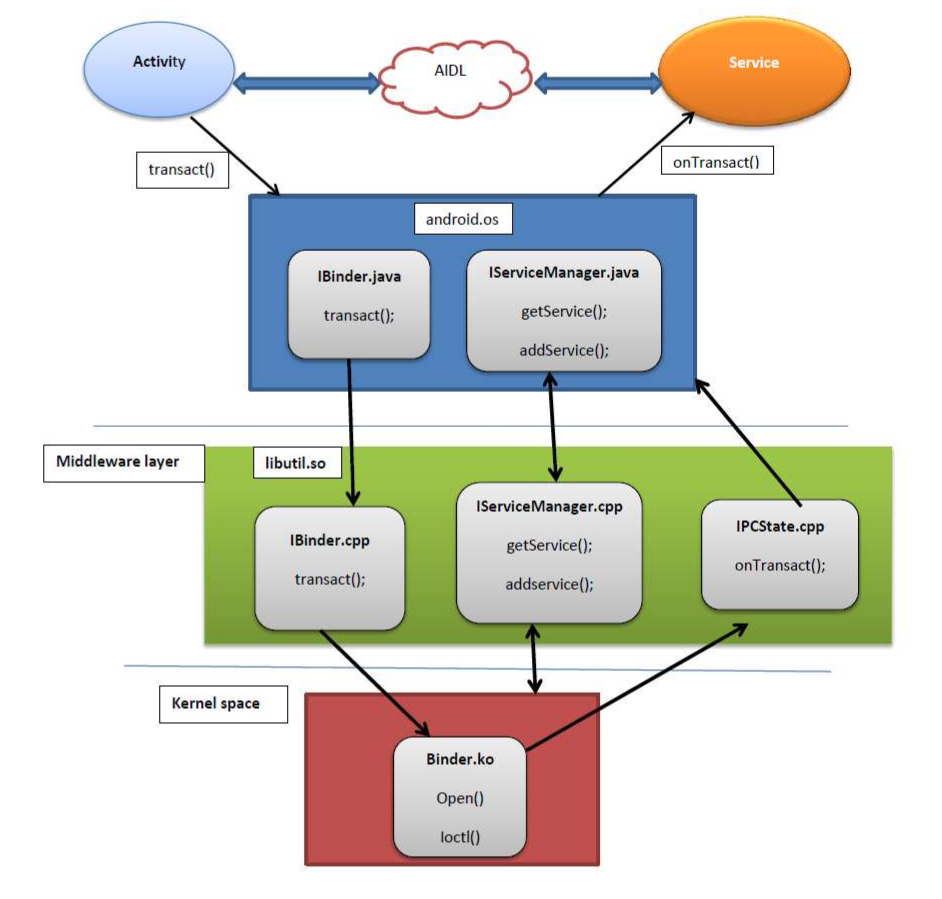
\includegraphics[width=0.9\textwidth]{src/img/binder/binderarch.png}
\caption{Binder Framework Architecture\cite{binder}}
\end{figure}

An example of a call to the service is provided to showcase how the argument marshalling and binder transaction are done in code.

\begin{minipage}{\linewidth}
\begin{lstlisting}[language=Java, caption=lockUserData service method, label=lst:lock-user-data-multi-user]
/**
 * Lock user data
 */
public int lockUserData(int userId)
                        throws RemoteException {
	Parcel _data = Parcel.obtain();
	Parcel _reply = Parcel.obtain();
	int _result;
	try {
		_data.writeInterfaceToken(DESCRIPTOR);
		_data.writeInt(userId);
		mRemote.transact(Stub.TRANSACTION_lockUserData, _data, _reply, 0);
		_reply.readException();
		_result = _reply.readInt();
	} finally {
		_reply.recycle();
		_data.recycle();
	}
	return _result;
}
\end{lstlisting}
\end{minipage}

\subsection{User Management and Interface}
\label{sub-sec:user-mngmt-inter-multi-user}

The second step is to make the relevant modifications in the framework in order to manage multiple encrypted users. Also, some changes to various Activities in the Settings Application need to be made.

The way multi-user Android systems work is that there is a separate data directory for each user and a separate media directory per user. This projects encrypts data directory, but it can be extended to the media directory as well.

The users are represented internally by integers. The default user(the owner) is user 0. Users created by the owner are identified by consecutive integers beginning with 10, with a limit of 8 users. Each user has a data folder in \texttt{/data/user/id}, where \text{id} is the integer representing that user.

\begin{minipage}{\linewidth}
\begin{lstlisting}[numbers=none, caption=User Data Directories, label=lst:usr-data-multi-user]
# ls -l /data/user/                                             
lrwxrwxrwx root     root              2000-03-11 17:07 0 -> /data/data/
drwxrwx--x system   system            2000-03-11 17:35 10
drwxrwx--x system   system            2000-03-11 17:37 11
\end{lstlisting}
\end{minipage}

An exception to this rule is the owner for which the data is stored in \texttt{/data/data} and \texttt{/data/user/0} is a link to this directory. This is mainly due to backwards compatibility requirements. For simplicity reasons, the project only handles encryption of  secondary users(those created by the owner).

To begin, the \texttt{UserInfo} class requires the addition of a flag that marks whether the user in question is encrypted.
\begin{lstlisting}[language=Java, numbers=none, caption=Encrypted User Flag, label=lst:encr-flag-multi-user]
/**
 * Encrypted
 */
public static final int FLAG_ENCRYPTED = 0x00000080;
\end{lstlisting}
The class constructor takes, among others, a \texttt{flags} parameter, which is an integer containing a bitwise or between several flags. The method for determining if a given user is encrypted using this parameter is the following.
\begin{lstlisting}[language=Java, numbers=none, caption=isEncrypted method, label=lst:encr-method-multi-user]
public boolean isEncrypted() {
	return (flags & FLAG_ENCRYPTED) == FLAG_ENCRYPTED;
}
\end{lstlisting}

Upon creation, the user is prompted with a dialog which asks whether the newly created user should be encrypted.

\begin{figure}[h!]
\centering
    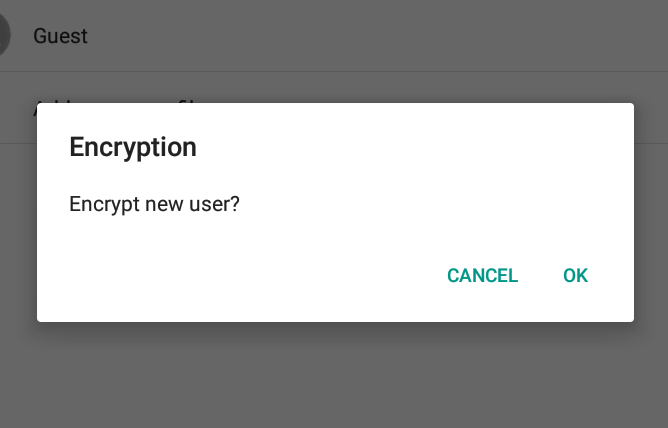
\includegraphics[width=0.9\textwidth]{src/img/multi-user/newuser.png}
\caption{User Creation}
\end{figure}

As mentioned in \labelindexref{Section}{sec:c-multi-user}, the user needs to provide a password which will be used to encrypt the master key. To avoid making the user creation process to cumbersome, instead of an extra dialog prompting for a user password, a default pin code \texttt{0000} is set for the new user. This can be modified by changing the password from the Settings Application.

Only one user may be active at any given time. When switching users, it is necessary to check whether the current user is encrypted. If this is the case, the user data directory needs to be locked. An example of doing this is presented below. This code is from the \texttt{UserSwitcherController} class. Highlighted in green are the additions made to the already existent code.

\lstdefinestyle{custom}{
	language=Java,
	basicstyle=\ttfamily\small,
	moredelim=**[is][\color{green!65!black}]{@}{@},
}

\begin{lstlisting}[style=custom]
private void switchToUserId(int id) {@
	final IBinder binder = ServiceManager.getService("efsservice");
	final int currentUser = ActivityManager.getCurrentUser();
	IEFSService service = null;
	if (binder != null && ambinder != null) {
		service = IEFSService.Stub.asInterface(binder);
	}@
	try {
		ActivityManagerNative.getDefault().switchUser(id);@
		if (service != null &&
		    mUserManager.getUserInfo(currentUser).isEncrypted())
			service.lockUserData(currentUser);@
	} catch (RemoteException e) {
		Log.e(TAG, "Couldn't switch user.", e);
	}
}
\end{lstlisting}

The same operation takes place when the device enters sleep mode either by the actioning of the power button or because the timeout set by the user expired. Shutting down the device does not need to be treated since when the device will be turned back on, the storage will not be mounted by default.

Similarly, when the user enters his password at the lockscreen, the storage corresponding to the data directory of the current user is unlocked.

The result is that, for each encypted user, the data directory is only ever unlocked starting the moment the user introduces the password and ending when the device is either switched to another user or in sleep or turned off.

\section{Issues}
\label{sec:issues-multi-user}

This chapter covers some of the issues encountered during the development of this project, as well as the issues that still remain. It is noteworthy that the project is a proof of concept and, therefore, is expected to have some shortcomings.

\subsection{SELinux}
\label{sub-sec:selinux-multi-user}

%http://selinuxproject.org/page/NB_Overview
The first of the issues is related to SELinux. SELinux is the primary Mandatory Access Control (MAC) mechanism built into a number of GNU/Linux distributions. SELinux operates using policies that define what access to resources and which operations on these resources are allowed. It is able to confine an application to its own domain, offering the minimum permissions required. It also assures that actions which are not allowed by policy are stopped, in order to attempt to prevent any damage.

To check wheter SELinux is running, the following command can be executed.
\begin{lstlisting}[numbers=none, caption=Checking SELinux status, label=lst:selinux-multi-user]
# getenforce
Enforcing
\end{lstlisting}
The result will be one of three values: \texttt{Enforcing, Permissive, Disabled}. \texttt{Enforcing} means SELinux is active and the policy will be applied. \texttt{Permissive} mode only logs actions that violate the policy, but will not prevent them. \texttt{Disabled} means SELinux is not active.

Given the fact that the project encrypts the data directory, it would require access permission to a wide range of files. Although SELinux offers a tool called \texttt{audit2allow} that transforms the output of the SELinux log into rules ready to be integrated into the policy, giving an application such extensive permissions is not recommended. Since the issue is beyond the scope of this project, a decision was made to disable SELinux during the development phase, thus simplifying the process.

\subsection{User Switching}
\label{sub-sec:user-switch-multi-user}

This issue was caused by how user switching works. Android users do not correspond directly to users in the underlying Linux system. Because of this, Android has more liberty in managing users. For example, in a classic Linux system, if a user has a password set, this password is requested at user switch. In Android, the password is requested at the lock screen, after the user switch has already taken place.

The actual issue arises from the fact that some applications attempt to access user data before the password is provided. Therefore, in the case of an encrypted user, these applications would try to access the data directory before it is mounted. For some of the applications, including the Launcher, this results in a crash.

For the purpose of this project, a workaround was used to circumvent this issue. When the password is entered, the user is stopped, the data directory is unlocked and then the user is started again. This way, the applications will be restarted and the data will be available. The proper method to deal with this problem would be to request a framework restart from the system. This, however, would incur restarting all users.

A small issue related to this one was that the crash messages for the applications would remain in the system queue and appear to the user even after the restart. This was solved by temporarily disabling dialogs between the user switch and the storage unlock.

\subsection{Miscellaneous}
\label{sub-sec:misc-mult-user}

Other, more minor issues still remain. Mostly, they are caused by simplifications used when developing. However, the proof of concept remains valid even with these issues present.

One issue was already mentioned: the fact that encryption of the owner is not permitted. This is a more complex case than the secondary users for a number of reasons:
\begin{itemize}
\item the encryption for the secondary users is done at creation, with no processes accessing the data directory; for the owner, the framework would need to be stopped
\item switching to the primary user would require the framework to be stopped, since user 0 cannot be stopped without doing so
\item the same as above applies for unlocking the device after it has been in sleep and the storage containing the data dir has been locked
\end{itemize}

Another shortcoming is the fact that encrypted users only work with PIN used for locking. Passwords are easy to integrate, since they would only require similar changes to those done for PIN codes. Patterns are also not an issue, since they are converted to a string internally, a string which can be used in place of a password for the storage. The only real issue is with more complex locking methods, like facial recognition.

One final issue to discuss is the what happens to background processes when the data directory is locked. In the current state, they crash as soon as an operation on a file from the data directory is attempted. This is a drawback for many applications. A possible fix would be something similar to what was presented in \labelindexref{Section}{sub-sec:and-priv-defreez}.

\section{Building}
\label{sec:build-multi-user}

This section describes the process of building the project using the emulator provided in AOSP(Android Open Source Project\abbrev{AOSP}{Android Open Source Project}). The emulator used will be the 64-bit version, but the 32-bit one can be used with the proper alteration of the instructions below. Note that some commands are too long to be written on a single line. Any line not starting from the far left should be treated as a continuation of the previous one. It is important to use the same branch of the AOSP repository, since the patches will most likely not apply to other versions. 

First, repo client has to be installed.

\begin{lstlisting}[numbers=none]
mkdir ~/bin
PATH=~/bin:$PATH
curl http://commondatastorage.googleapis.com/git-repo-downloads/repo > ~/bin/repo
chmod a+x ~/bin/repo
\end{lstlisting}

Next, in order to download the AOSP source code:
\begin{lstlisting}[numbers=none]
AOSP_TREE=$PWD/AOSP
mkdir $AOSP_TREE
cd $AOSP_TREE
repo init -u https://android.googlesource.com/platform/manifest -b android-5.0.2_r1
repo sync -j8
\end{lstlisting}

The next step is to download the project source code and apply the integration patches:
\begin{lstlisting}[numbers=none]
git clone https://github.com/catalinionita/Ecryptfs-Tools-for-Android.git $AOSP_TREE/external/efs-tools
cd $AOSP_TREE
external/efs-tools/integration/apply_patches.sh
\end{lstlisting}

The build environment needs to be setup. The steps to install all required packages for different Linux distributions are in the AOSP wiki.\footnote{\url{http://source.android.com/source/initializing.html\#setting-up-a-linux-build-environment}}

To build the Android tree and the emulator:
\begin{lstlisting}[numbers=none]
source build/envsetup.sh
lunch aosp_x86_64-eng
make update-api
make -j8
\end{lstlisting}

Next, the kernel is required and eCryptfs support needs to be enabled:
\begin{lstlisting}[numbers=none]
git clone https://android.googlesource.com/kernel/goldfish.git $AOSP_TREE/goldfish-kernel
cd $AOSP_TREE/goldfish-kernel
git checkout android-goldfish-3.10
\end{lstlisting}

To start with the default configuration for the x64 kernel:
\begin{lstlisting}[numbers=none]
make ARCH=x86_64 x86_64_emu_defconfig
\end{lstlisting}

The following lines need to be added to the configuration file. Edit \$AOSP_TREE/goldfish-kernel/.config
\begin{lstlisting}[numbers=none]
CONFIG_KEYS=y
CONFIG_CRYPTO=y
CONFIG_CRYPTO_ALGAPI=y
CONFIG_CRYPTO_BLKCIPHER=y
CONFIG_CRYPTO_HASH=y
CONFIG_CRYPTO_MANAGER=y
CONFIG_CRYPTO_MD5=y
CONFIG_CRYPTO_ECB=y
CONFIG_CRYPTO_CBC=y
CONFIG_CRYPTO_AES=y
CONFIG_ECRYPT_FS=y
\end{lstlisting}
To disable SELinux support, comment the line beginning with \texttt{CONFIG_SECURITY_SELINUX} in the same file.

To build the kernel, the cross-compiler path must be set.
\begin{lstlisting}[numbers=none]
export CROSS_COMPILE=$AOSP_TREE/prebuilts/gcc/linux-x86/x86/x86_64-linux-android-4.9/bin/x86_64-linux-android-
make ARCH=x86_64 CC="${CROSS_COMPILE}gcc -mno-android" bzImage
\end{lstlisting}

Once the kernel has been built, the emulator can be started as follows:
\begin{lstlisting}[numbers=none]
 emulator -kernel $AOSP_TREE/goldfish-kernel/arch/x86/boot/bzImage -skin WXGA800-7in -prop fw.max_users=8 -prop fw.show_multiuserui=1 -qemu -m 1024 -enable-kvm
\end{lstlisting}
It will start a 7 inch emulator with multi-user support. See all emulator options on the developer wiki.\footnote{\url{http://developer.android.com/tools/help/emulator.html}}

To check that the C library is functional, the test suite included in the source code repository can be used.
\begin{lstlisting}[numbers=none]
$AOSP_TREE/external/efs-tools/test/testsuite.sh
\end{lstlisting}

Testing multi-user encryption is not automated at this point. However, \texttt{adb shell} can be used to connect to the device. Once connected, to check whether a storage is mounted or not, the \texttt{mount} command is used.

\begin{lstlisting}[numbers=none, style=custom]
# mount
rootfs / rootfs ro,seclabel,relatime 0 0
tmpfs /dev tmpfs rw,seclabel,nosuid,relatime,mode=755 0 0
devpts /dev/pts devpts rw,seclabel,relatime,mode=600 0 0
proc /proc proc rw,relatime 0 0
sysfs /sys sysfs rw,seclabel,relatime 0 0
selinuxfs /sys/fs/selinux selinuxfs rw,relatime 0 0
debugfs /sys/kernel/debug debugfs rw,relatime 0 0
none /acct cgroup rw,relatime,cpuacct 0 0
none /sys/fs/cgroup tmpfs rw,seclabel,relatime,mode=750,gid=1000 0 0
tmpfs /mnt/asec tmpfs rw,seclabel,relatime,mode=755,gid=1000 0 0
tmpfs /mnt/obb tmpfs rw,seclabel,relatime,mode=755,gid=1000 0 0
none /dev/cpuctl cgroup rw,relatime,cpu 0 0
/dev/block/platform/sdhci-tegra.3/by-name/APP /system ext4 ro,seclabel,relatime,user_xattr,acl,barrier=1,data=ordered 0 0
/dev/block/platform/sdhci-tegra.3/by-name/CAC /cache ext4 rw,seclabel,nosuid,nodev,noatime,errors=panic,user_xattr,acl,barrier=1,nomblk_io_submit,data=ordered 0 0
/dev/block/platform/sdhci-tegra.3/by-name/UDA /data ext4 rw,seclabel,nosuid,nodev,noatime,errors=panic,user_xattr,acl,barrier=1,nomblk_io_submit,data=ordered 0 0
/dev/fuse /mnt/shell/emulated fuse rw,nosuid,nodev,relatime,user_id=1023,group_id=1023,default_permissions,allow_other 0 0@
/data/user/.10 /data/user/10 ecryptfs rw,seclabel,relatime,ecryptfs_fnek_sig=180e26f6e1e174f8,ecryptfs_sig=81661eb0fc6a797b,ecryptfs_cipher=aes,ecryptfs_key_bytes=32 0 0@
\end{lstlisting}

The highlighted line corresponds to an unlocked storage for user 10. The absence of this line would mean the directory is locked.